\documentclass[a4paper]{article}
\usepackage[T1]{fontenc}
\usepackage[utf8]{inputenc}
\usepackage[english,italian]{babel}
\usepackage{amsfonts}
\usepackage{amsmath}
\usepackage{amsthm}
\usepackage{graphicx}
\usepackage{listings}
\lstset{upquote=true}
\graphicspath{ {./} }
\begin{document}
\author{Alessio Susco mat. 266383}
\title{Report progetto Ingegneria degli Algoritmi}
\maketitle
\theoremstyle{definition}
\newtheorem{definition}{Definition}[section]
\newtheorem{theorem}{Theorem}
\section{Introduzione}
Al giorno d'oggi, moltissime sono le applicazioni che fanno uso intensivo di algoritmi per il calcolo di cammini minimi su grafi. Il problema principale dei grafi nelle applicazioni moderne è che cambiano la loro struttura continuamente ed in modo non predicibile a priori. Gli eventi che vanno a cambiare la struttura del grafo possono essere: aggiunta o rimozione di nodi e/o archi e incrementi/decrementi dei pesi degli archi.
L'obiettivo di questo studio è quello di andare a valutare le performance di due algoritmi per il calcolo dei cammini minimi di un grafo a fronte di eventi di aggiunta di archi ed incremento dei pesi degli archi.
I due algoritmi presi in esame sono quelli messi a disposizione dal toolkit Networkit nella libreria distance, in particolare: distance.Dijkstra e distance.DynDijkstra.
\subsection{DynDijkstra}
L'algoritmo DynDijkstra, dato un grafo e un evento, permette di calcolare i cammini minimi da un nodo sorgente andando a ricalcolare solo i cammini che sono stati influenzati dall'evento.
\subsection{Dijkstra}
L'algoritmo Dijkstra, dato un grafo, permette di calcolare i cammini minimi da un nodo sorgente.
Al contrario del precedente appena descritto è intuibile che ,a fronte di tali eventi, è necessario rieseguirlo per avere i cammini minimi corretti ed aggiornati. 
Pertanto, tale algoritmo è stato utilizzato per quantificare quanto fosse più veloce l'algoritmo dinamico in particolari set di grafi.
\section{Progettazione degli esperimenti}
Con questo studio si vuole determinare come varia lo speedup tra l'algoritmo statico e quello dinamico al variare delle taglie dei grafi in input, pertanto per la scelta dei fattori e dei design points si è fatto riferimento alle linee guida relative alle categorie di domande di tipo Assessment.
Di seguito verranno brevemente riportate le metriche ed i parametri scelti:
\begin{itemize}
\item Performance Metrics: Speedup e Time
\item Performance Indicator: CPU Time speso dai due algoritmi, scelta obbligata per ridurre al minimo l'influenza degli altri processi sui risultati durante l'elaborazione
\item Algorithm Parameters: istanze di grafi e nodo sorgente (Dijkstra(graph, source)). Inoltre, anche gli eventi di modifica delle istanze dei grafi sono stati considerati come parametri algoritmici
\item Instance Parameters: 
\begin{itemize}
\item Input Source: I grafi sono stati generati randomicamente da due classi di generatori, cioè ErdosRenyi e BarabasiAlbert
\item Input Size: $n$: numero dei nodi, $p$: probabilità dell'esistenza di un arco per i grafi ER e $k$:numero di archi uscenti da un nodo per i grafi BA
\end{itemize}
\item Factors: I parametri che vengono esplicitamente manipolati nei seguenti esperimenti sono
il numero dei nodi nei grafi. In particolare, i livelli sono stati scelti seguendo la logica del Doubling Experiment partendo da un valore iniziale abbastanza grande che permettesse di evitare risultati spuri dovuti al floor effect. Il numero di raddoppi è stato scelto come compromesso tra generalità dei risultati, somiglianza a taglie di grafi dinamici reali e tempi di sperimentazione accettabili.
\item Fixed Parameters: Il numero di eventi di modifica del grafo durante gli esperimenti è fissato a priori. Inoltre, anche $p$ e $k$ (parametri di istanza) sono stati fissati. In particolare $p=0.02$ per i grafi Erdos-Renyi è stato scelto in modo da soddisfare le ipotesi di un teorema che ci garantisce che la probabilità del grafo generato $P(\{G(n,p) \quad is connected\})\rightarrow 1$
\item Noise Parameters: Il tipo di evento dinamico di modifica del grafo è scelto casualmente ma in modo semicontrollato dato che i possibili eventi sono due, ovvero l'aggiunta di un arco al grafo e l'incremento del peso di un arco già presente nel grafo. Anche i pesi degli archi vengono scelti randomicamente tra due valori fissati a priori. Per diminuire il bias statistico dovuto al nodo sorgente, è stato scelto di cambiare, ad ogni evento, il nodo sorgente per il calcolo dei cammini minimi..
\item Design Points: Date 6 taglie di input per ogni grafo
\[n = (500,1000,2000,4000,8000,16000)\]
e due tipologie di grafi \[GraphType = (BarabasiAlbert, ErdosRenyi)\] abbiamo ottentuto 12 design points
\end{itemize}
\section{Test Environment}
In questo paragrafo verranno riportate tutte le implementazioni e gli script necessari all'esecuzione degli esperimenti precedentemente descritti con l'obiettivo di riassumere il loro funzionamento.
L'intero ambiente di test è rappresentato dal seguente workflow:\\
\begin{figure}[!h]
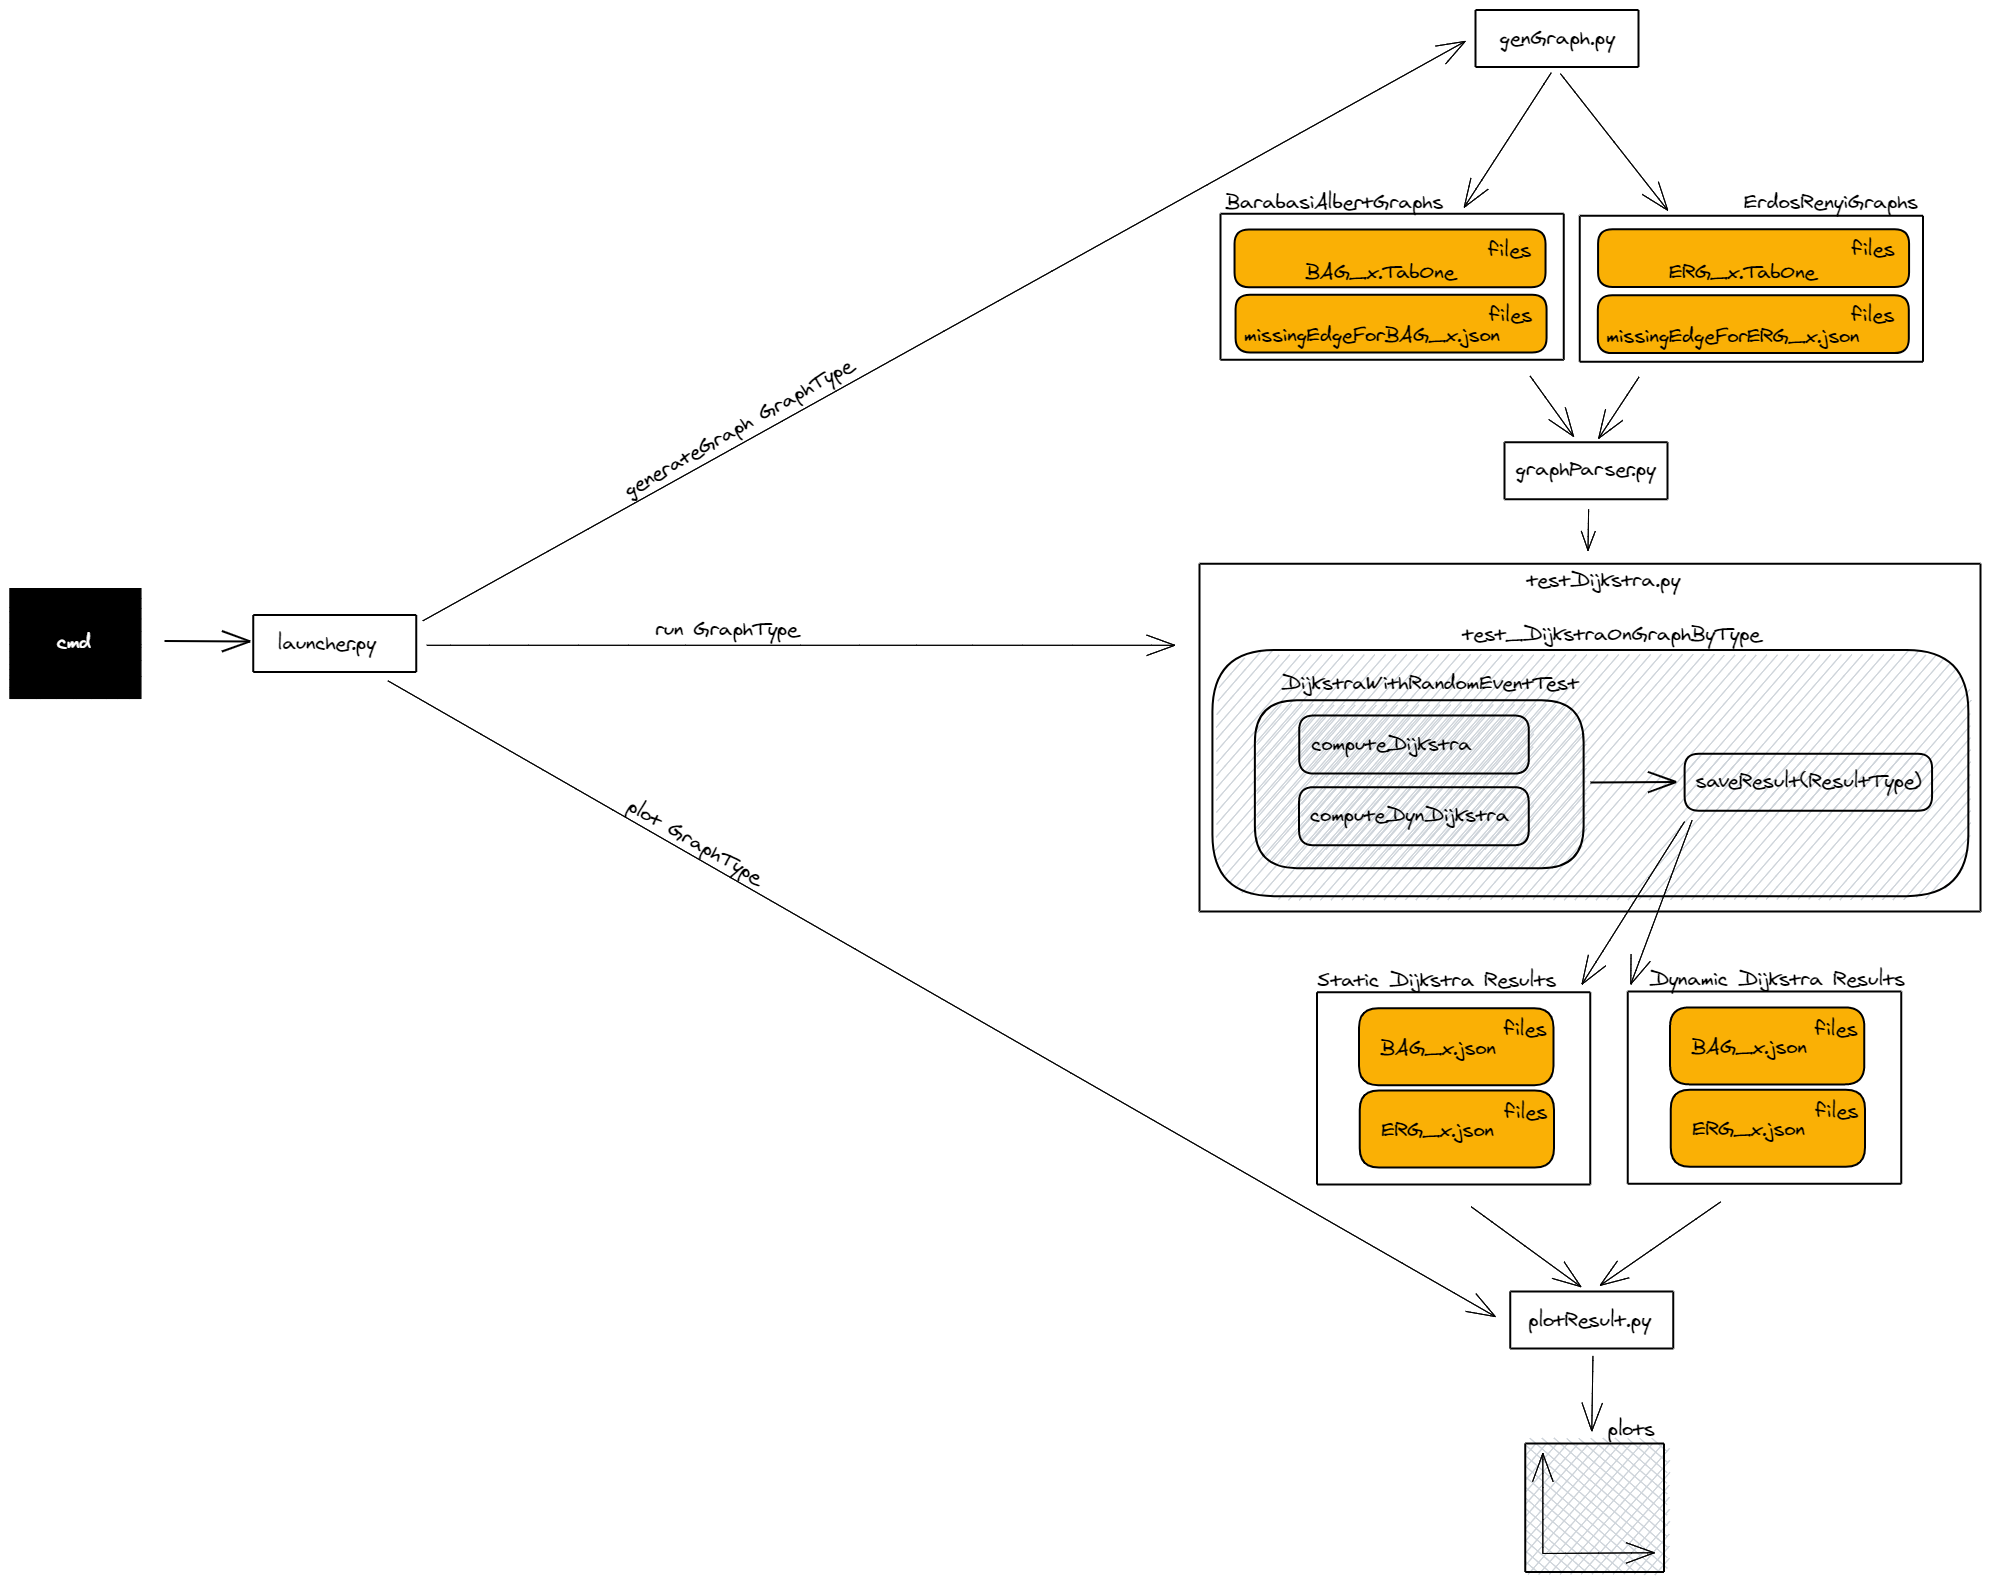
\includegraphics[scale=0.17]{img/workflow}
\centering
\caption{Test Enviroment Workflow}
\end{figure}
\newpage
\subsection{Implementazioni}
E' possibile eseguire i test attraverso lo script python $launcher.py$ con i seguenti comandi:
\begin{itemize}
\item -h per visualizzare i comandi
\item -g GraphType per generare i grafi del tipo GraphType
\item -r GraphType per eseguire i test dei due algoritmi sui grafi di tipo GraphType precedentemente generati
\item -p GraphType per plottare i risultati ottenuti dall'esecuzione dei test
\end{itemize}
E' presente un ulteriore script chiamato $utility.py$ nel quale sono presenti funzioni comuni tra i vari script e parametri di settings dell'intero ambiente di test e verranno descritti successivamente. E' necessario anticipare la presenza in $utility.py$ di:
\begin{itemize}
\item path relativi delle folder nelle quali vengono salvati i grafi e i risultati dell'esecuzione dei test
\item enum $GraphTypes$ per identificare i tipi di grafi
\item enum $DijkstraAlgoTypes$ per identificare l'algoritmo statico o dinamico
\end{itemize}
\newpage
\subsubsection{Phase 1 Graph Generation}
\begin{figure}[!h]
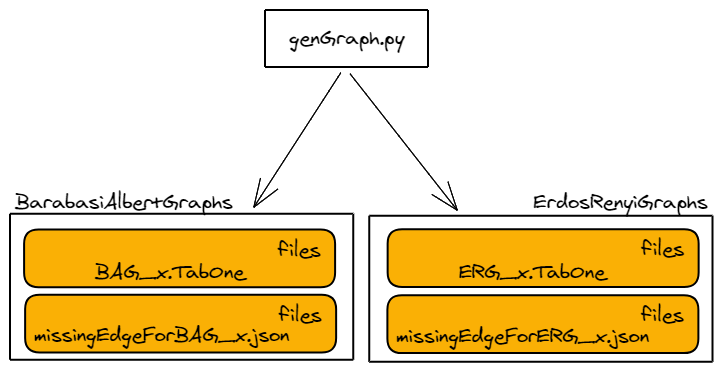
\includegraphics[scale=0.35]{img/01_cmd_to_graphFiles}
\centering
\caption{Phase 1: cmd to graphFiles}
\end{figure}
Lo script $genGraph.py$ si occupa di generare i grafi e salvarli su file. 
Per la generazione dei grafi vengono utilizzati i seguenti parametri di input presenti nello script $utility.py$:
\begin{itemize}
\item $MIN\_NODES$ : numero minimo di nodi
\item $MIN\_K$ : numero minimo di collegamenti per ogni nodo (parametro di input per la generazione dei grafi di Barabasi-Albert
\item $MIN\_PROB$ : probabilità minima dell'esistenza di un arco (parametro di input per la generazione dei grafi di Erdos-Renyi
\item $N\_GRAPH$ : numero di grafi da generare attraverso il doubling, ovvero il numero di volte che viene raddoppiato il numero di nodi del grafo da generare
\end{itemize}
Per ogni grafo così generato verranno calcolati gli archi mancanti attraverso un semplice algoritmo random e ad ognuno di essi verrà assegnato un peso randomico compreso tra due valori definiti dalle seguenti variabili presenti nello script $utility.py$, cioè:
\begin{itemize}
\item $MIN\_EDGE\_WEIGHT$
\item $MAX\_EDGE\_WEIGHT$
\end{itemize}
I grafi generati verranno salvati su file, attraverso metodi dedicati offerti dalla libreria networkit, in formato $.TabOne$. Invece gli archi mancanti, con i relativi pesi, verranno salvati in formato $.json$.
La folder nella quale verranno salvati è configurabile nello script $utility.py$ con le variabili:
\begin{itemize}
\item $BAGs\_FOLDER$ : folder nella quale verranno salvati i grafi di tipo Barabasi-Albert in formato $.TabOne$
\item $ERGs\_FOLDER$ : folder nella quale verranno salvati i grafi di tipo Erdos-Renyi in formato $.TabOne$
\end{itemize}
E' stato necessario adottare tale strategia di generazione e salvataggio in quanto il tempo di generazione dei grafi era di poco inferiore al tempo di esecuzione dell'esperimento e ciò ha permesso un notevole risparmio di tempo nella sperimentazione degli algoritmi oggetto di studio.
Proprio grazie al risparmio di tempo recuperato dalla fase di generazione dei grafi è stato possibile aumentare notevolmente la taglia degli stessi mantenendo un tempo di sperimentazione accettabile.
\subsubsection{Phase 2 Graph Deserialize}
\begin{figure}[!h]
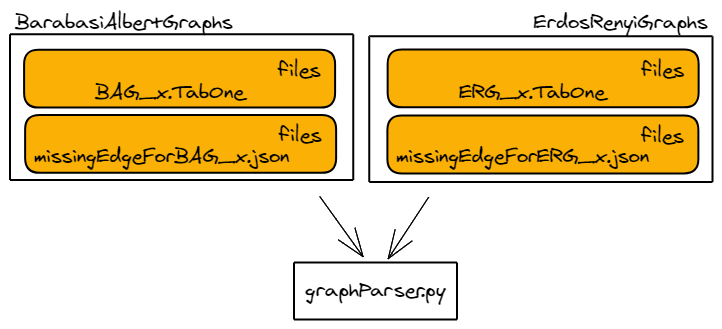
\includegraphics[scale=0.4]{img/02_graphFiles_to_graphParser}
\centering
\caption{Phase 2: graphFiles to graphParser}
\end{figure}
Affinché i grafi e gli archi mancanti, salvati nella fase precedente, fossero utilizzabili è stato necessario implementare dei metodi di lettura da file. Per fare ciò è stata creata una classe di appoggio chiamata $GraphParser$ e utilizzabile importando lo script $graphParser.py$. Tale oggetto si occupa di leggere da file, ricostruire e restituire al chiamante una lista così costituita: $[indice, grafo, lista\_archi\_mancanti]$ relativa al $GraphType$ passato in input.
\newpage
\subsubsection{Phase 3 Run Test Dijkstra Algorithms}
\begin{figure}[!h]
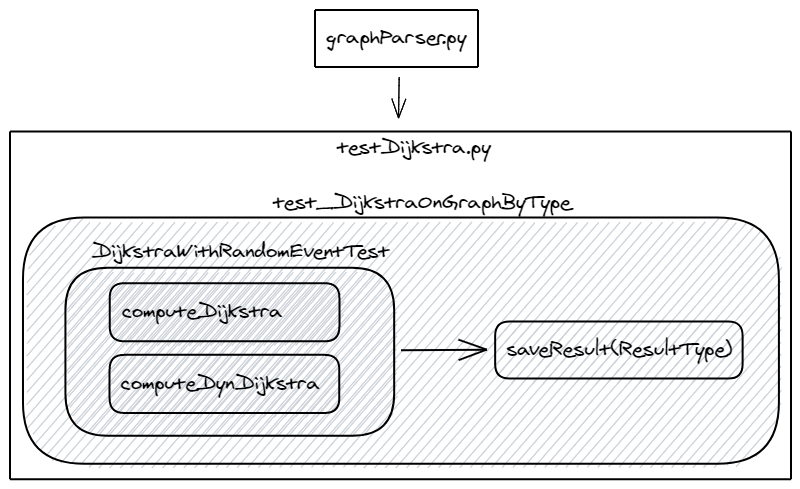
\includegraphics[scale=0.43]{img/03_graphParser_to_testDijkstra}
\centering
\caption{Phase 3: graphParser to testDijkstra}
\end{figure}
Lo script $testDijkstra.py$ implementa il core di questo studio sperimentale. In particolare si occupa di eseguire l'algoritmo di Dijkstra e l'algoritmo DynDijkstra sui grafi precedentemente generati. Il flusso della sperimentazione è il seguente:
\begin{figure}[!h]
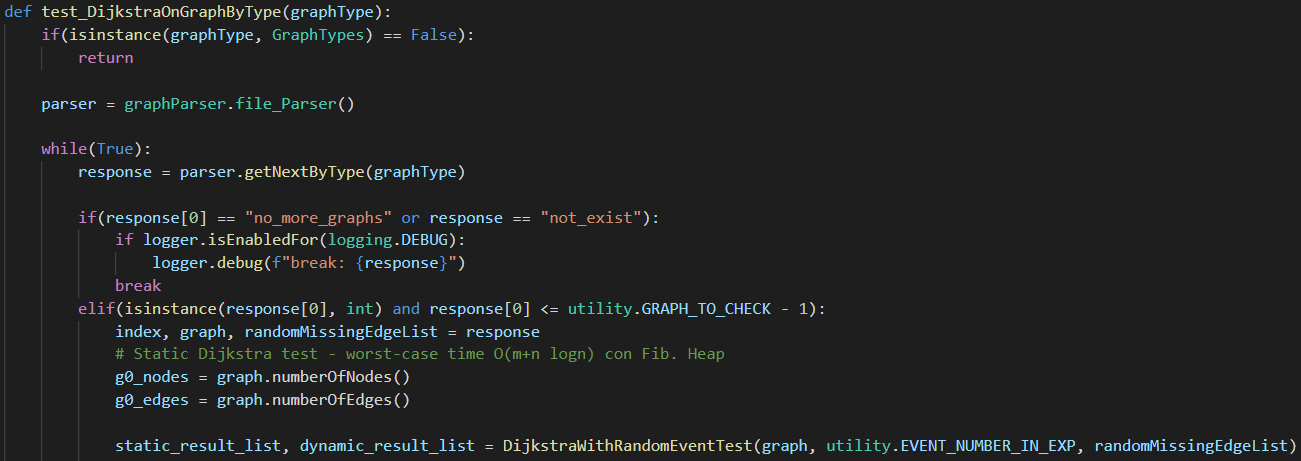
\includegraphics[scale=0.35]{img/test_DijkstraOnGraphByType}
\centering
\caption{test\_DijkstraOnGraphByType function}
\end{figure}
\begin{itemize}
\item Viene creato l'oggetto graphParser precedentemente illustrato
\item Viene eseguita la function DijkstraWithRandomEventTest finchè il graphParser trova grafi generati in precedenza e tali grafi vengono passati alla funzione. Un ulteriore input è il numero di esperimenti. Tale numero rappresenta la quantità di eventi di aggiunta di archi o decremento del peso di archi esistenti del grafo ed è un parametro fisso configurabile nello script $utility.py$
\end{itemize}
\newpage
\begin{figure}[!h]
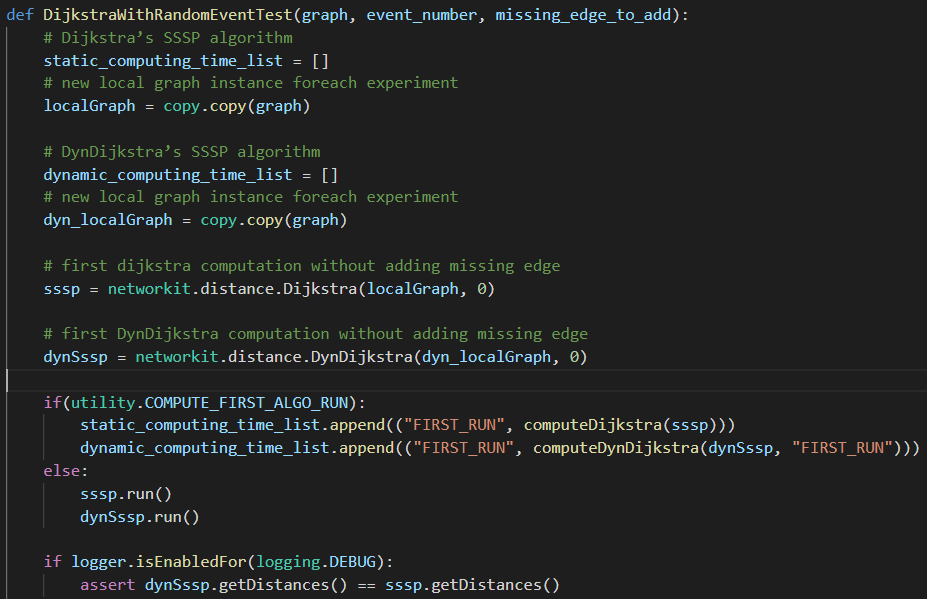
\includegraphics[scale=0.47]{img/01_DijkstraWithRandomEventTest}
\centering
\caption{DijkstraWithRandomEventTest function}
\end{figure}
La prima parte della funzione DijkstraWithRandomEventTest si occupa di 
\begin{itemize}
\item allocare le strutture dati contenenti i grafi
\item eseguire gli algoritmi di Dijkstra su tali grafi
\end{itemize}
Questa esecuzione non viene presa in considerazione in quanto, essendo la prima, sia l'algoritmo dinamico che quello statico impiegano lo stesso tempo e dunque non aggiungono informazioni utili al test.
\newpage
\begin{figure}[!h]
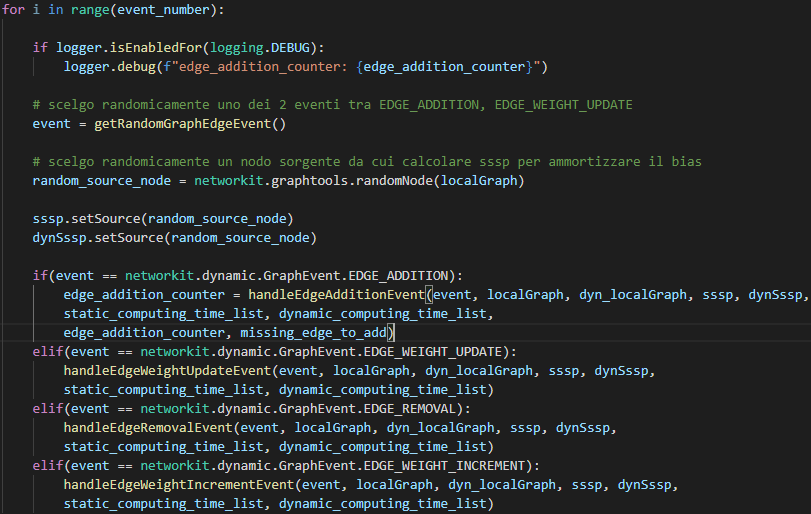
\includegraphics[scale=0.56]{img/02_DijkstraWithRandomEventTest}
\centering
\caption{DijkstraWithRandomEventTest function}
\end{figure}
La seconda parte della funzione DijkstraWithRandomEventTest si occupa invece di
\begin{itemize}
\item scegliere randomicamente tra due possibili eventi di modifica del grafo 
\item scegliere randomicamentre il nodo sorgente, dal quale verrà effettuato Single Source Shortest Path, tra tutti i possibili nodi del grafo. Tale scelta è stata fatta per evitare il bias statistico causato dal nodo sorgente, ovvero per evitare che la casualità degli eventi di modifica del grafo rendessero meno oneroso il calcolo da parte dell'algoritmo DynDijkstra da nodo sorgente fisso
\item gestire l'evento scelto randomicamente attraveso i rispettivi metodi handle
\end{itemize}
\newpage
\begin{figure}[!h]
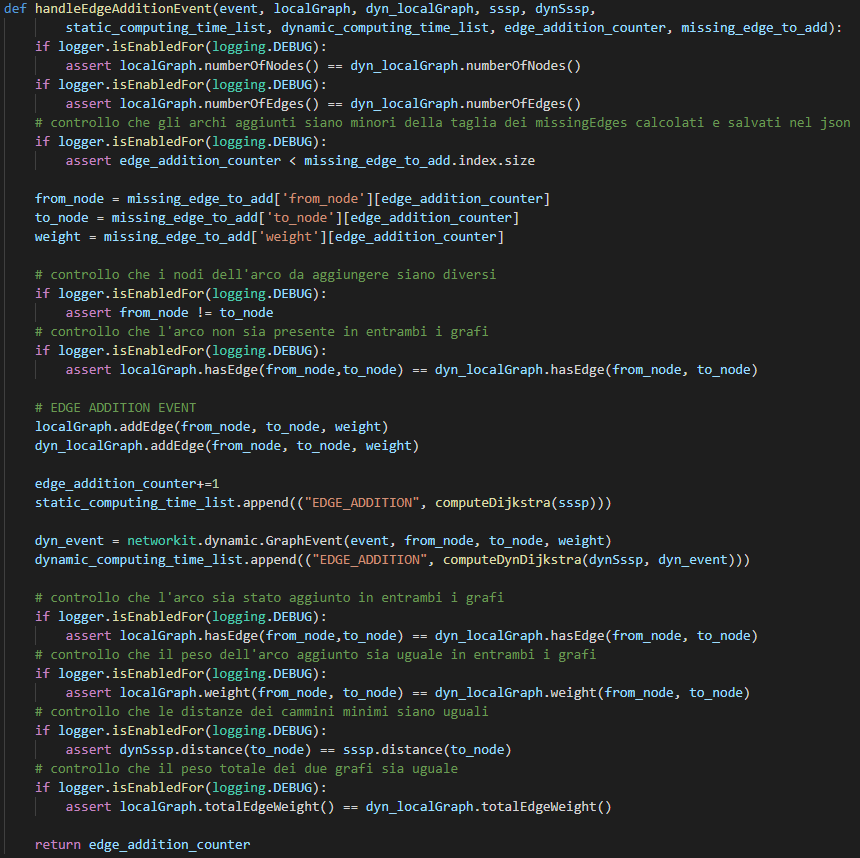
\includegraphics[scale=0.52]{img/handleEdgeAdditionEvent}
\centering
\caption{handleEdgeAdditionEvent function}
\end{figure}
Le funzioni handle si occupano di gestire i vari eventi di modifica del grafo e nel seguito verrà presentato il funzionamento della function che gestisce l'evento di aggiunta di un arco nel grafo. In particolare, si occupa di
\begin{itemize}
\item prendere un arco dalla lista di archi mancanti letta in precedenza da file
\item aggiungere tale arco al grafo
\item eseguire le funzioni $computeDijkstra$ e $computeDynDijkstra$ le quali si occupano di 
eseguire i rispettivi algoritmi e restituire il tempo di esecuzione impiegato per tale computazione. Per evitare che la misura fosse influenzata da interrupt di sistema e altri processi presenti nella macchina sulla quale sono stati eseguiti i test è stato scelto di utilizzare come metro di misura il CPU time.
\end{itemize}
Ulteriori precisazioni sono necessarie riguardo la correttezza e l'efficienza dei test.
Per quanto riguarda la correttezza è sono state utilizzate in modo intensivo le assertion le quali hanno permesso di verificare la correttezza dei passaggi per le modifiche sul grafo. Inoltre è stato possibile validare i risultati dei due algoritmi asserendo che le distanze da loro calcolate dovessero essere necessariamente uguali. Proprio attraverso la validazione effettuata è stato possibile scoprire che l'algoritmo DynDijkstra oggetto di test non gestisce correttamente l'evento di incremento del peso e di rimozione di un arco restituendo distanze dei cammini minimi non corrette. Per tale motivo è stato necessario limitare il test di tale algoritmo agli eventi di aggiunta di un arco e decremento del peso di un arco. Per quanto riguarda l'efficienza dei test, l'uso intensivo delle assertion e delle print su console ha avuto un impatto molto negativo sul tempo di esecuzione. Per tale motivo è stato utilizzata utilizzata una libreria python per implementare il sistema di logging. Quando il logger è settato in modalità DEBUG è possibile osservare i print su console per valutare il comportamento del test a runtime e assicurarci tramite le assertion che l'ambiente di test funzioni correttamente. Invece quando il logger è configurato in modalità INFO vengono saltati i passaggi precedentemente descritti e questo ha portato ad un risparmio notevole soprattutto sui running time dei due algoritmi. Di seguito i tempi di esecuzione dell'intero test (generazione, esecuzione, plot) nelle configurazioni rispettivamente di DEBUG e INFO eseguiti su 6 grafi Erdos-Renyi con numero di nodi (500, 1000, 2000, 4000, 8000, 16000) e 35000 eventi eseguiti per ogni grafo:
\begin{figure}[!h]
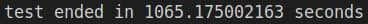
\includegraphics[scale=1]{img/test_DEBUG_6g_500n_35Kevent_20KmissingEdge}
\centering
\caption{running time with logger in DEBUG mode}
\end{figure}
\begin{figure}[!h]
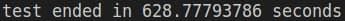
\includegraphics[scale=1]{img/test_INFO_6g_500n_35Kevent_20KmissingEdge}
\centering
\caption{running time with logger in INFO mode}
\end{figure}
\newpage
\subsubsection{Phase 4 Serialize Test Data}
\begin{figure}[!h]
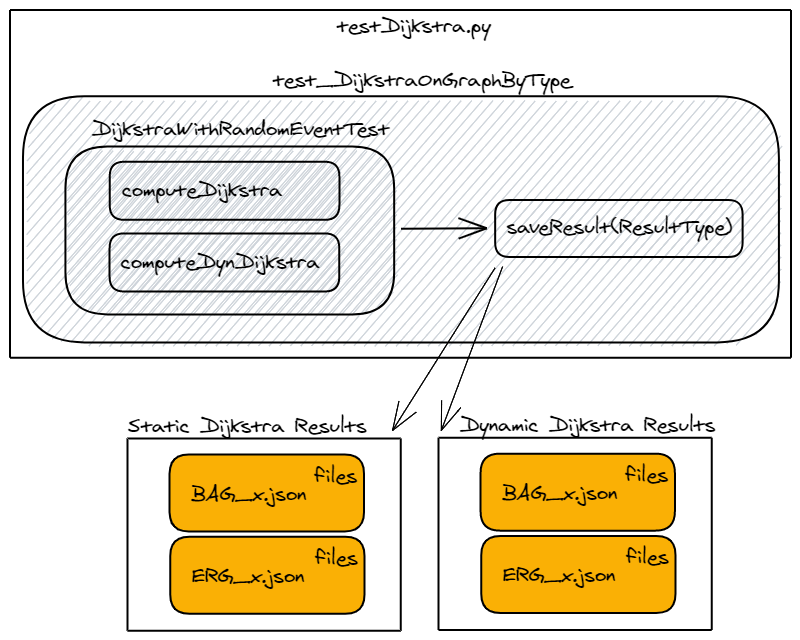
\includegraphics[scale=0.4]{img/04_testDijkstra_to_resultFiles}
\centering
\caption{Phase 4: testDijkstra to resultFiles}
\end{figure}
Alla fine dell'esecuzione della funzione $DijkstraWithRandomEventTest$ verranno restituite due liste, contenenti rispettivamente i running time impiegati dall'algoritmo di Dijkstra e DynDijkstra, le quali verranno salvate su file insieme alle informazioni relative alla sperimentazione effettuata. In particolare, verranno generati due file in formato json, uno per ogni tipo di algoritmo eseguito, contenenti le seguenti informazioni:
\begin{itemize}
\item graph\_type: GraphType
\item graph\_number: index
\item nodes: numero di nodi del grafo
\item edges: numero di archi del grafo
\item total\_weight: peso totale del grafo
\item result\_list: lista contenente tutti i running time dell'algoritmo per ogni evento di aggiunta/decremento del peso
\end{itemize}
\newpage
\subsubsection{Phase 5 Plot Results}
\begin{figure}[!h]
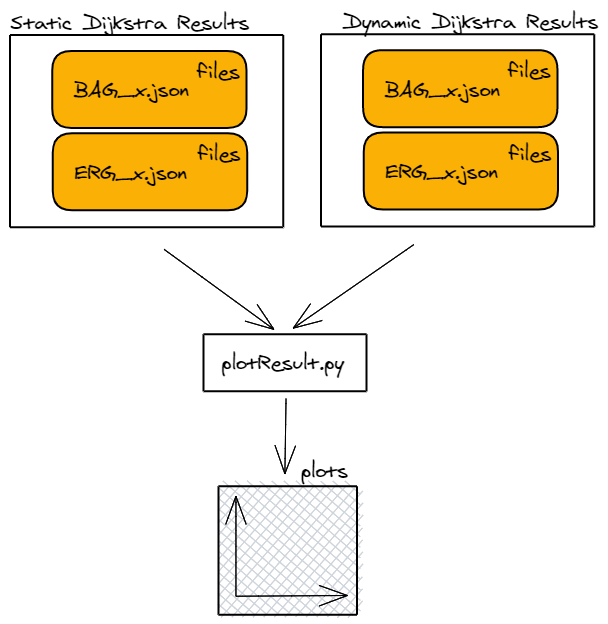
\includegraphics[scale=0.4]{img/05_resultFiles_to_plots}
\centering
\caption{Phase 5: resultFiles to plots}
\end{figure}
Lo script $plotResult.py$ si occupa di leggere i file json generati dai test, manipolare tali dati e plottare i grafici opportuni che verranno discussi nel paragrafo successivo. La separazione in fasi del test enviromment ha consentito lo sviluppo e la validazione degli script senza la necessità di attendere il tempo necessario all'elaborazione degli algoritmi.
\newpage
\section{Risultati}
I risultati sono stati ottenuti eseguendo gli esperimenti su un notebook con le seguenti caratteristiche hardware:
\begin{itemize}
\item CPU Intel Core i9-9980HK (8 Core, 16 Thread, 5Ghz)
\item GPU NVIDIA GeForce GTX 1650 (4 GB GDDR5)
\item RAM 16 GB DDR4 2666MHz
\item Disco a stato solido M.2 2230/2280 (PCIe Gen3.0x4 NVMe, 32 Gb/s)
\end{itemize}
Al fine di quantificare l'efficienza dell'algoritmo di Dijkstra dinamico rispetto a quello statico, verranno di seguito riportati i grafici dei risultati ottenuti dai test precedentemente illustrati.
In particolare verranno distinti i risultati ottenuti eseguendo i due algoritmi su grafi generati secondo Barabasi-Albert da Erdos-Renyi.

Per prima cosa, per validare i due algoritmi, è stato confrontato il running time dei due algoritmi con la complessità nota in letteratura (in termini asintotici).
Sono stati riportati due grafici all'interno della stessa figura. Il primo per evidenziare la differenza dei running time tra i due algoritmi. Il secondo per vedere quale andamento ha il running time dell'algoritmo dinamico, che a causa dei diversi ordini di grandezza con quello statico, non è ben comprensibile dalla prima figura.
\begin{figure}[!h]
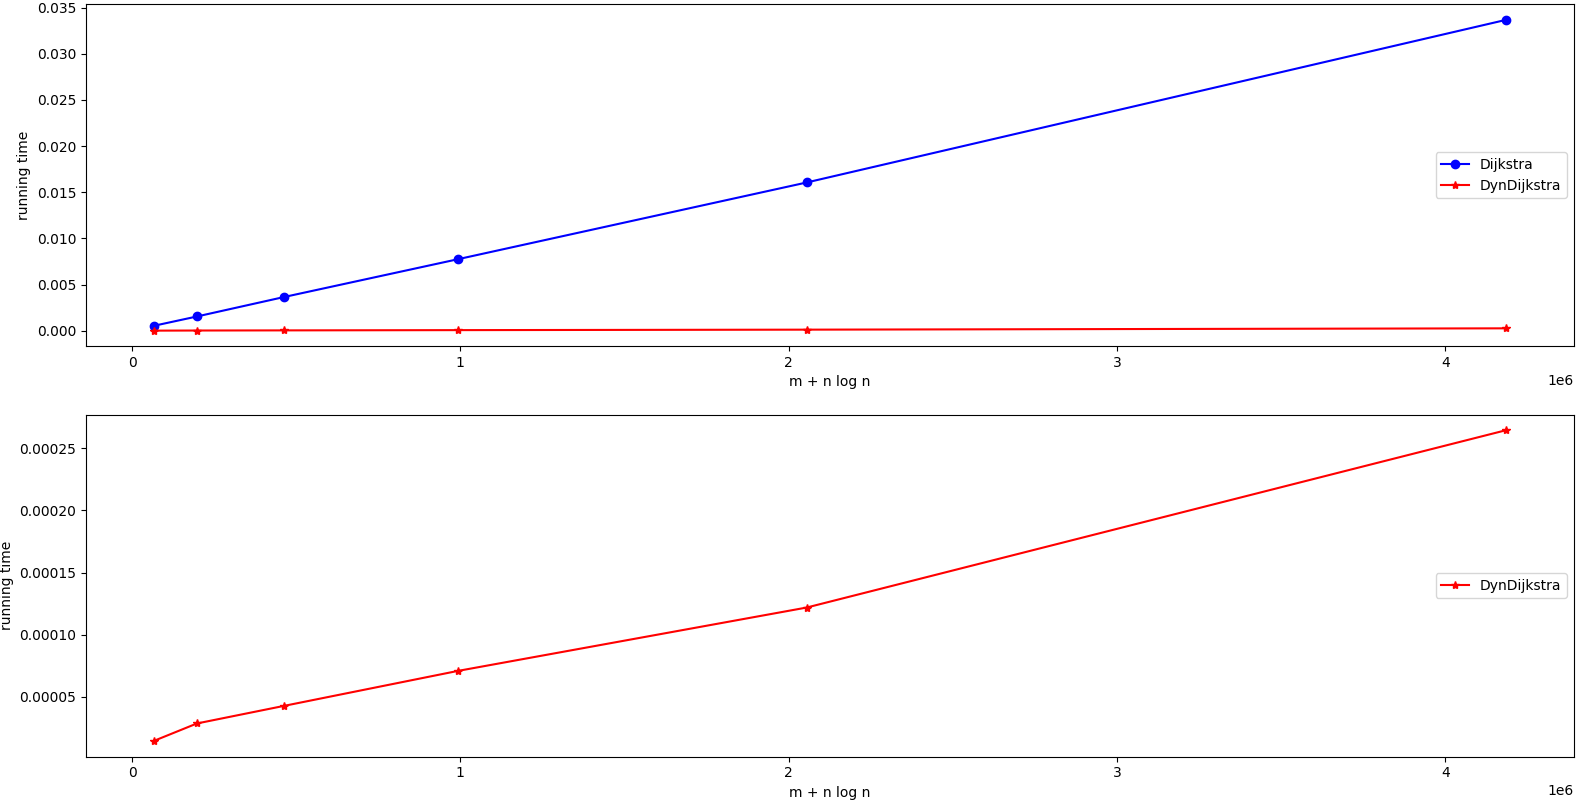
\includegraphics[scale=0.29]{img/BAG_F1_ExpectedAsymptotic-RunningTime}
\centering
\caption{Barabasi-Albert Graph: Asymptotic Comparison}
\end{figure}
\begin{figure}[!h]
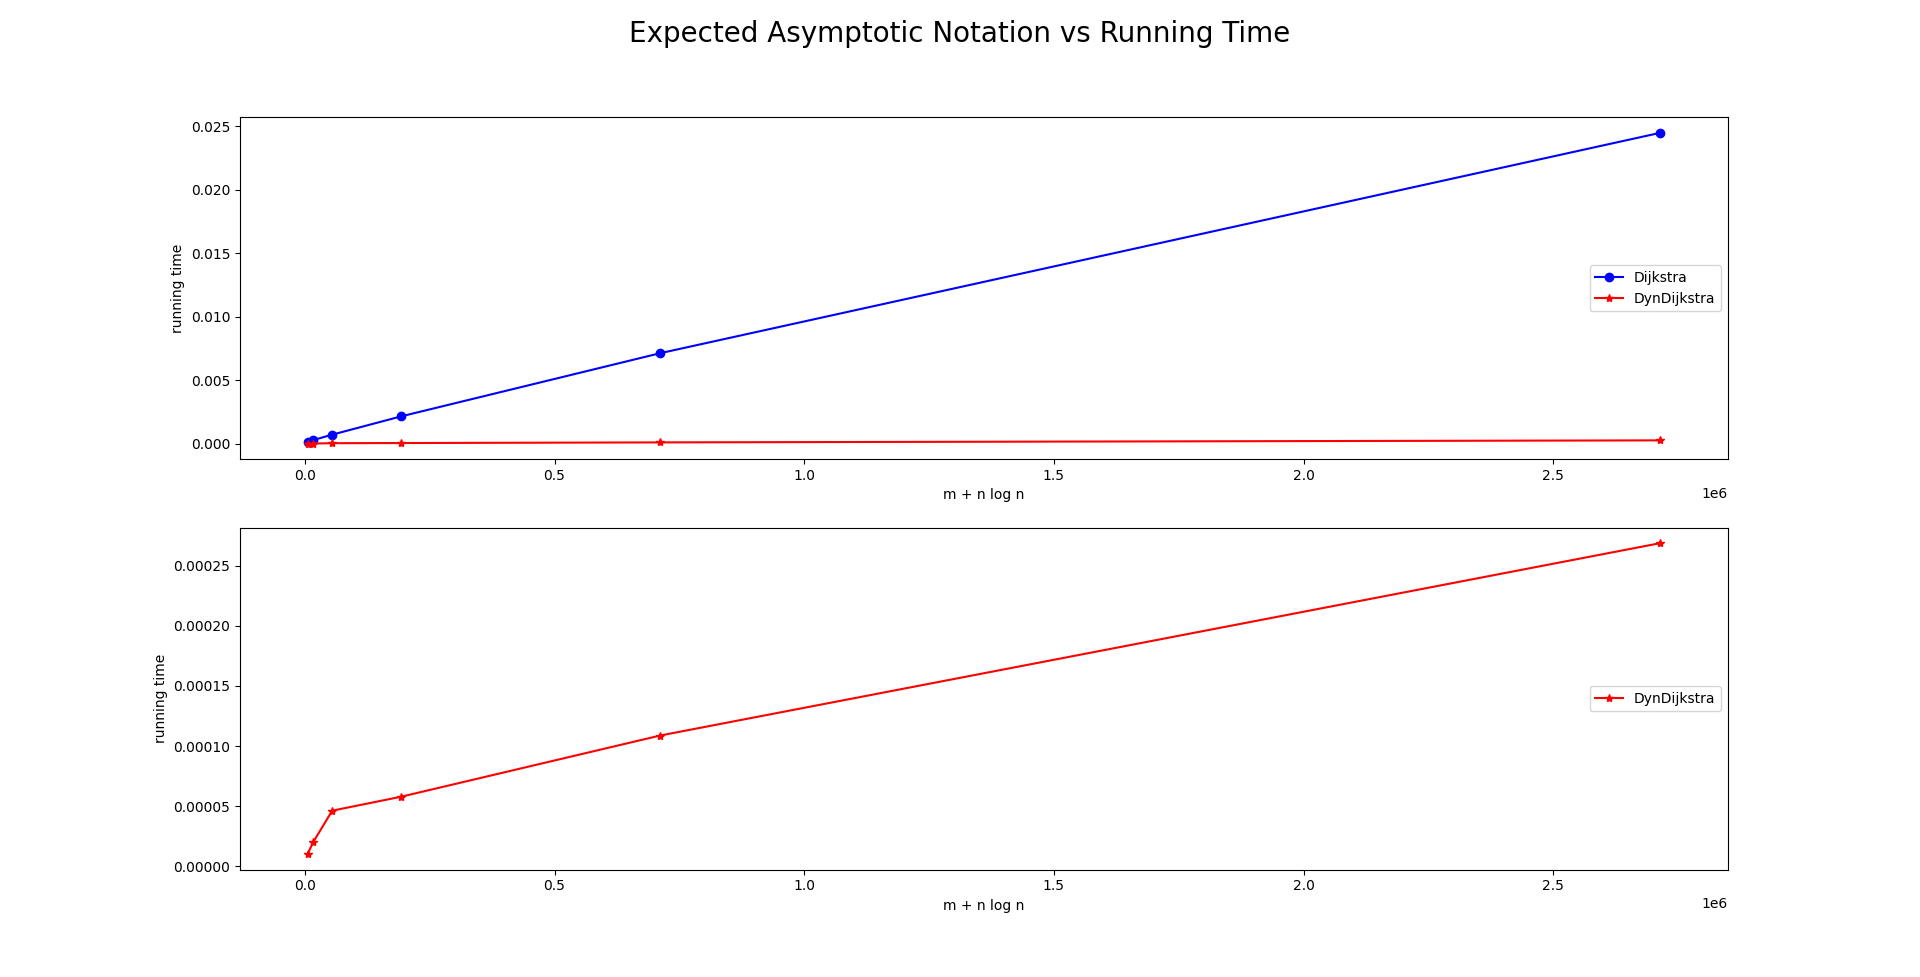
\includegraphics[scale=0.29]{img/ERG_F1_ExpectedAsymptotic-RunningTime}
\centering
\caption{Erdos-Renyi Graph: Asymptotic Comparison}
\end{figure}
\newpage
Successivamente è stato ritenuto opportuno osservare come lo speedup varia al variare del numero dei nodi del grafo. In particolare il numero dei nodi del grafo è stato scelto attraverso la tecnica del doubling experiment.
\begin{figure}[!h]
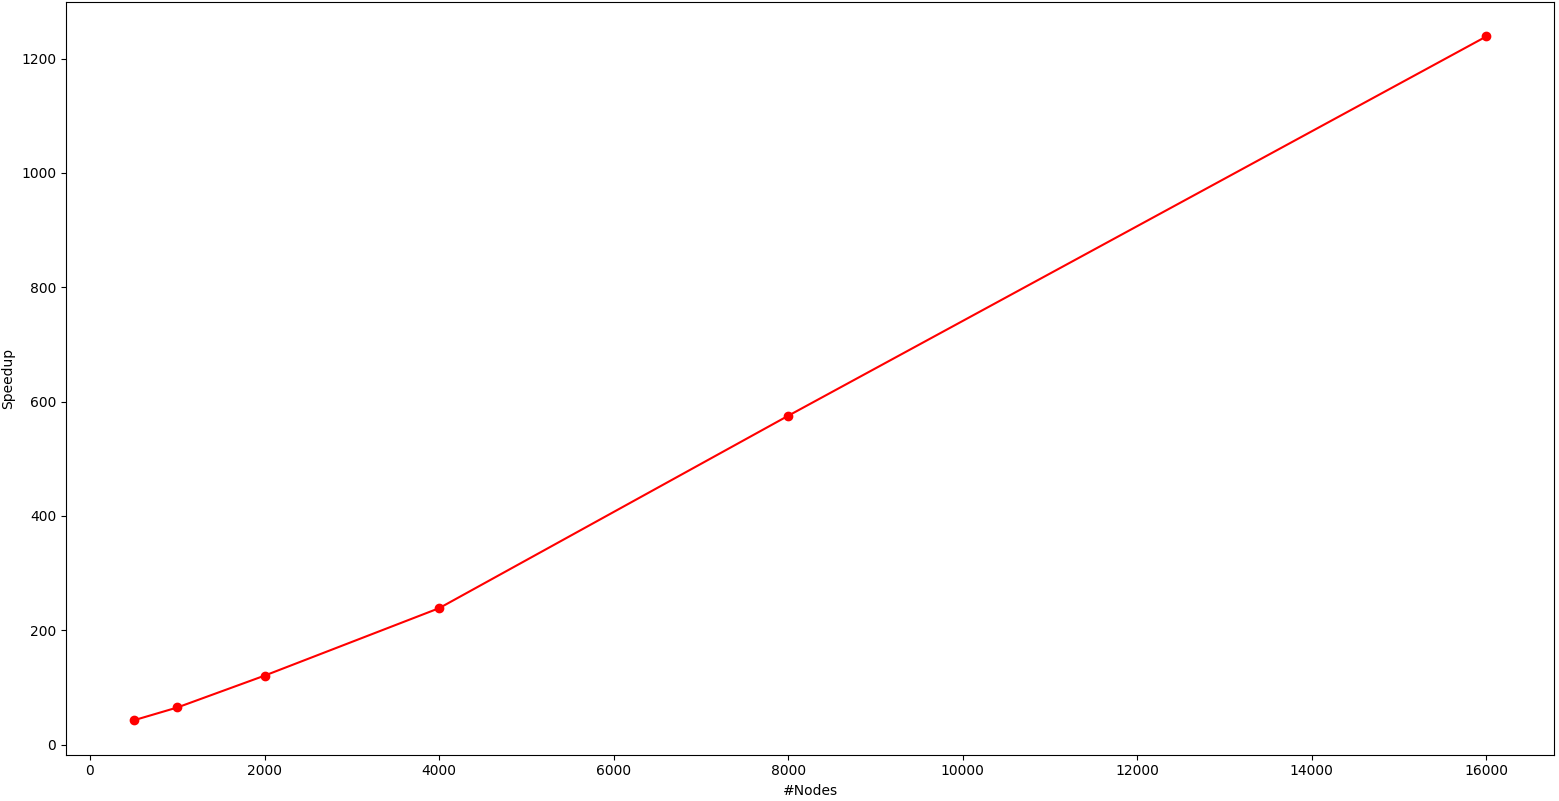
\includegraphics[scale=0.29]{img/BAG_F2_Nodes-Speedup}
\centering
\caption{Barabasi-Albert Graph: \#Nodes vs Speedup}
\end{figure}
\begin{figure}[!h]
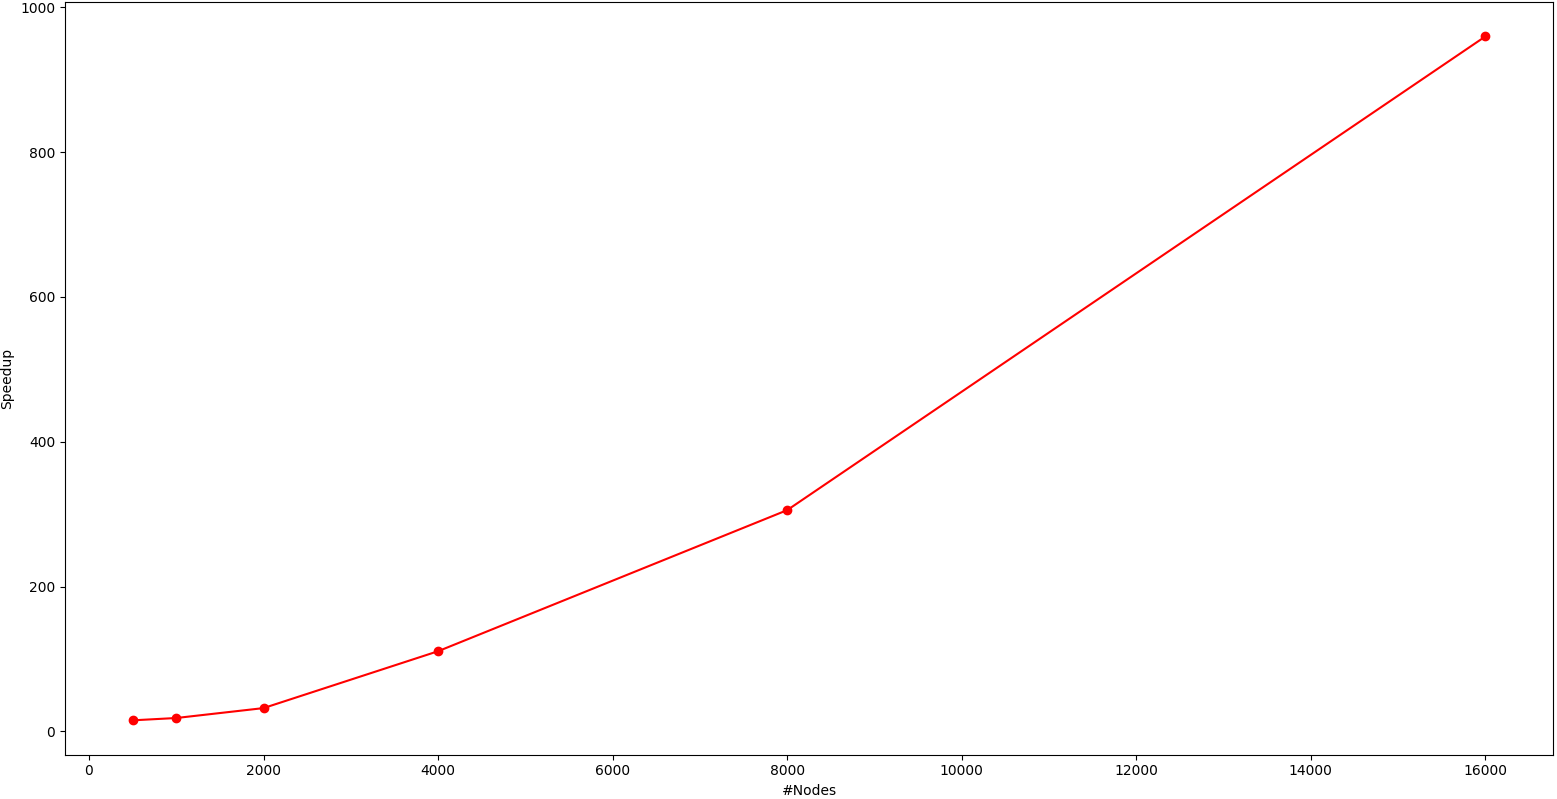
\includegraphics[scale=0.29]{img/ERG_F2_Nodes-Speedup}
\centering
\caption{Erdos-Renyi Graph: \#Nodes vs Speedup}
\end{figure}
\newpage
Infine è stato utilizzato un modello di regressione polinomiale per stabilire l'andamento dello speedup tra i due algoritmi. Ogni punto arancione in figura rappresenta lo speedup tra i due algoritmi ad ogni evento di modifica del grafo. In particolare, per ogni taglia di grafo, sono stati eseguiti esattamente 35000 eventi riportati nell'ordine in cui si sono succeduti. 
\begin{figure}[!h]
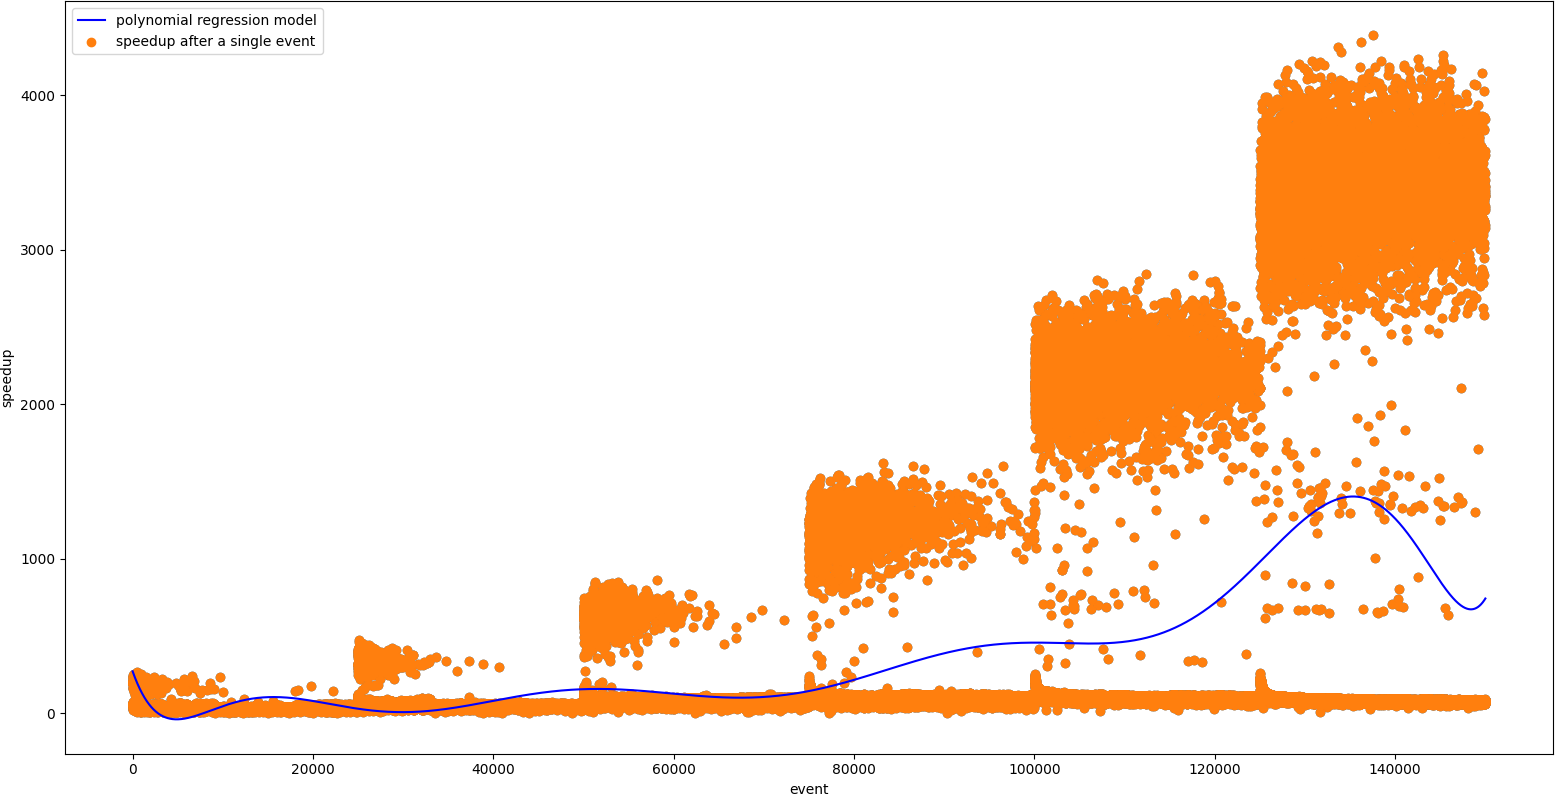
\includegraphics[scale=0.29]{img/BAG_F3_Event-Speedup}
\centering
\caption{Barabasi-Albert Graph: event vs Speedup}
\end{figure}
\begin{figure}[!h]
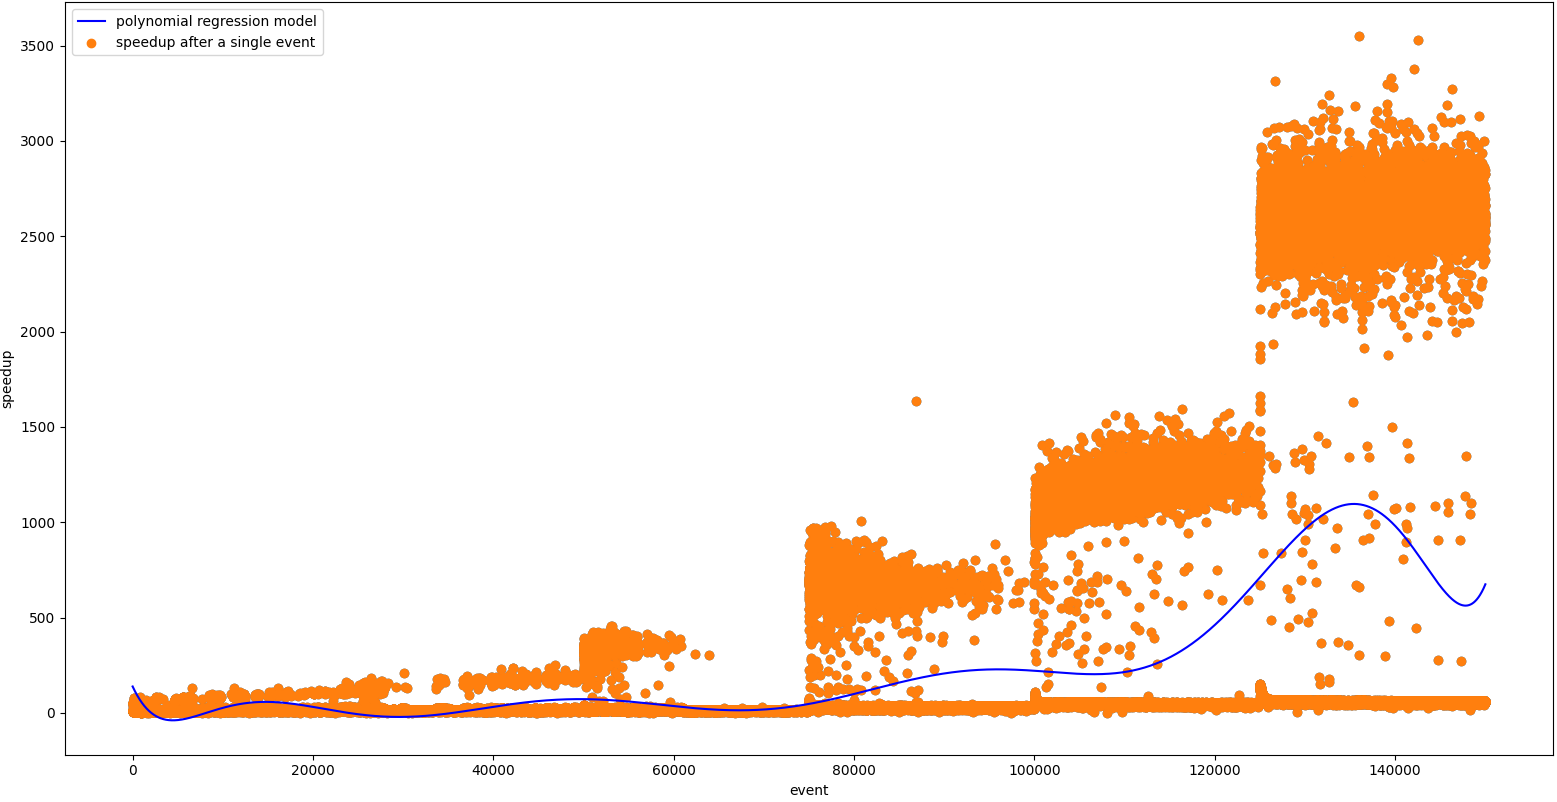
\includegraphics[scale=0.29]{img/ERG_F3_Event-Speedup}
\centering
\caption{Erdos-Renyi Graph: event vs Speedup}
\end{figure}
\newpage
\section{Conclusioni e sviluppi futuri}
Dall'analisi dei risultati ottenuti è possibile concludere, limitatamente agli
esperimenti condotti, che:
\begin{itemize}
\item Lo speedup tra i due algoritmi varia dal trascurabile a tre ordini di grandezza
\item L'algoritmo dinamico, seppur molto più veloce in determinate situazioni, presenta comunque un andamento tipico di Dijkstra che varia da sublineare a quadratico in base alla densità del grafo
\item dalla figura 15 e 16 non vi è una differenza sufficiente per concludere che i grafi Barabasi-Albert e Erdos-Renyi influenzano l'andamento dell'algoritmo dinamico rispetto a quello statico. Nonostante ciò, si può comunque concludere che lo speedup aumenta in modo lineare all'aumentare dei nodi di un grafo purché non aumenti in modo rilevante la densità.
\item Il numero di eventi di modifica rispetto alla grandezza del nodi del grafo ne influenza in modo significativo l'andamento. In particolare:
- Aggiungere molti archi in un grafo piccolo fa decrescere lo speedup. A conferma del fatto che in un grafo completo lo speedup dei due algoritmi è circa uguale se non negativo (a causa del fatto che l'algoritmo dinamico avrà un'overhead dovuto all'identificazione delle variazioni).
- Al crescere delle dimensioni dei grafi lo speedup aumenta (mediamente) come già visto in precedenza ma , dalle figure 17 e 18, emergono dati importanti circa la distribuzione degli eventi molto, poco e mediamente onerosi in termini di tempo. In particolare, ci sono eventi a causa dei quali l'algoritmo dinamico deve ricalcolare tutto esattamente come quello statico. Infatti, ci sono eventi al di sotto dello 0 nell'asse delle ascisse proprio perchè, a fronte di quell'evento, l'algoritmo dinamico è stato addirittura più lento di quello statico.
- E' intuibile ma non dimostrabile con certezza attraverso i dati ottenuti che lo speedup crescerà fino al suo massimo teorico nel caso di un grafo completo a fronte di un singolo evento ottimo ma mediamente tenderà a scendere man mano che si ci si avvicina alle condizioni di completezza.
\end{itemize}
Questi risultati offrono quel minimo di dati che consentono di fare delle scelte guidate, quantificandone a priori i risultati che sarà possibile ottenere, li dove vi è l'esigenza di scegliere tra l'enorme complessità di implementazione di un algoritmo dinamico e l'accontentarsi di determinati running time a vantaggio di una complessità di implementazione minore.

Eventuali sviluppi futuri potrebbero essere:
\begin{itemize}
\item ripetere i test con particolari e contestualizzati set di grafi
\item parallelizzare i test su più core e/o dispositivi li dove possibile
\item approfondire la ricerca di caratteristiche determinanti e/o correlazioni tra parametri attraverso studi workhorse mirati
\end{itemize}
\end{document}